\part{Impianti a vapore}
\begin{adjustwidth}{2in}{}
	Un altro impianto utilizzato per la generazione di energia è l'impianto a vapore. 
	
	L'impianto a vapore è un sistema a circuito chiuso e in quanto tale permette di espandere a pressioni minori di quella atmosferica, ciò consente un aumento del lavoro estratto dalla turbina. 
	
	In più, a valle dell'impianto, attraverso le pompe di estrazione del condensato e quella di alimento, viene compresso liquido e non gas:
	\[dl = \dfrac{dP}{\rho} \qquad\qquad \rho_\text{liquido}\sim1000\cdot\rho_\text{gas}\]
	Questo comporta un minor lavoro di compressione richiesto al sistema e quindi un lavoro netto estraibile maggiore, e in aggiunta non si verifica il problema del lavoro di controrecupero. 
	
	SCHEMA DETTAGLIATO
	
	In cui si possono sempre individuare i seguenti punti
	\begin{itemize}
		\item[5)] Liquido saturo alla pressione del condensatore in uscita dal condensatore
		\item[0)] Liquido saturo alla pressione ambiente in entrata alla pompa di alimento $P_\text{al}$
		\item[1')] Liquido sottoraffreddato alla pressione del generatore di vapore
		\item[1)] Liquido saturo alla pressione del generatore di vapore in uscita dall'economizzatore
		\item[2)] Vapore saturo alla pressione del generatore di vapore
		\item[3)] Vapore surriscaldato alla pressione del generatore di vapore
		\item[4)] Vapore espanso alla pressione del condensatore				
	\end{itemize}
	
	Poiché ogni ciclo ha bisogno di una sorgente calda e di una sorgente fredda per adempiere al proprio scopo, il condensatore fa la parte della sorgente fredda, dove viene sottratto calore, mentre il generatore di vapore (nel suo insieme) fa la parte della sorgente calda, quella dove viene immesso calore. \newline 
	
	Nei piani termodinamici di maggior interesse il ciclo che rappresenta l'impianto a vapore è il ciclo Hirn/Rankine
	
	DISEGNI
	
	In questo caso il diagramma di Mollier rende possibile - anche per via grafica - il calcolo delle proprietà termodinamiche del fluido nonché dei lavori di pompa e di turbina.
\end{adjustwidth}



\section{Criteri generali di massimizzazione del rendimento e del lavoro specifico}
\begin{adjustwidth}{2in}{}
	È possibile controllare la temperatura e la pressione al generatore di vapore e la pressione al condensatore. \newline
	
	Tuttavia la trasformazione termodinamica all'interno di quest'ultimo componente è caratterizzata da varianza unitaria: c'è passaggio di fase; ciò significa che al condensatore data una temperatura sarà per forza fissata una pressione e viceversa. Allora dato che non è possibile scendere al di sotto della temperatura ambiente {\footnotesize (a meno di dover fornire lavoro al ciclo che non è conveniente se il fine è la produzione)}, l'unico vincolo variabile sul lavoro estratto diviene quello della temperatura al condensatore. 
	
	Ciò è un vincolo variabile perché la temperatura ambiente è essa stessa variabile. \newline
	
	Solitamente si mantiene un $\Delta T \simeq 10\degree C$, ciò permette infatti di minimizzare quanto più possibile la pressione al condensatore, tuttavia questa soluzione rimane realizzabile solamente per grandi impianti a vapore raffreddati ad acqua fluviale, e richiedono dai 50 ai 60 kg di acqua di raffreddamento per kg di vapore, il che si porta dietro scambiatori di calore dell'elevato costo e ingombro.
	
	Se invece si sceglie di raffreddare ad aria, essendo questo un aeriforme serviranno maggiori sezioni di passaggio e maggiori portate d'aria di raffreddamento: la soluzione che si adopera è quella delle torri evaporative. 
\end{adjustwidth}



\subsection{Ottimizzazione del generatore di vapore}
\begin{adjustwidth}{2in}{}
	Dal ciclo \textbf{Rankine} (Hirn senza surriscaldamento) è possibile individuare la posizione ottimale di del punto $P$ che massimizza il calore fornito, $L$ che massimizza il lavoro estratto ed $\eta$ che massimizza il rendimento termodinamico del ciclo.  
	
	DISEGNO
	
	Innanzitutto si traslano gli assi sul punto $0$ in modo da far combaciare 
	\[\begin{cases}
		y = \Delta h\\
		x = \Delta s
	\end{cases}\]
	In questo modo il \underline{calore} fornito al ciclo diviene rappresentabile come una funzione che plotti la curva limite superiore del ciclo 
	\[h_P-h_0 = y(x)\]
	La posizione del punto che massimizza il calore sarà così dato da 
	\[\dfrac{dy(x)}{dx} = 0\]
	Ed è il punto $Q$, in cui la tangente alla curva è una retta orizzontale. 
	
	Si trova che 
	\[P_Q = 4~\text{MPa} \qquad T_Q = 250~\degree C\]
	
	Similmente, per massimizzare il \underline{lavoro}, si scrive 
	\[l = q_1-q_2 = (h_P-h_0) - (h_A-h_0) = y(x) - T_Kx \]
	La quantità $(h_A-h_0)$ è il calore prelevato al condensatore, questa quantità sul diagramma $h$ è rappresentabile come una retta passante per l'origine di pendenza $T$. 
	
	Anche in questo caso la condizione di massimo lavoro si trova attraverso
	\[\dfrac{dl}{dx} = 0 \Rightarrow \dfrac{dy(x)}{dx} = T_K\]
	Ovvero il punto $L$ che massimizza il lavoro è l'intersezione tra la curva limite superiore e la tangente alla curva limite superiore parallela alla retta OA.
	
	Si trova che, se al condensatore
	\[P_K = 5~\text{kPa} \qquad T_k = 32~\degree C \quad \Rightarrow \quad P_L = 12.5~\text{MPa}\]
	
	Allo stesso modo, per il \underline{rendimento}, essendo
	\[\eta = \dfrac{l}{q_1} = \dfrac{y(x)- T_Kx}{y(x)} = 1-\dfrac{T_Kx}{y(x)}\]
	Derivando si ottiene 
	\[\dfrac{dy(x)}{dx} = \dfrac{y}{x}\]
	Il punto $\eta$ che massimizza il rendimento è l'intersezione tra la curva limite superiore e la retta tangente alla curva limite superiore parallela alla bisettrice del primo quadrante.
	
	Si trova che 
	\[P_{\eta} = 18.6~\text{MPa}\]
	
	Parimenti per il ciclo \textbf{Hirn}, il vincolo sulla temperatura massima è fornito da fattori puramente tecnologici, generalmente si raggiungono
	\[T_{\max}=[500\div600]~\degree C\]
	Avere generatori di vapore e turbine che operino a temperature maggiori è economicamente sconveniente, il basso incremento di lavoro che si otterrebbe non basta a ripagare il costo delle avanzate tecnologie utilizzate. 
	
	Poiché si effettua il surriscaldamento e dato che l'isobara di surriscaldamento ha sempre una concavità verso l'alto, il \underline{calore} fornito al fluido è sempre crescente per cui non è necessario adoperarsi per trovare un massimo. 
	
	Il \underline{lavoro}, come nel ciclo Rankine, diviene massimizzabile fissata una $T_{\max}$: la $P_{\max}$ è infatti quella per la quale la tangente nel punto di vapore saturo sarà parallela alla retta del condensatore. 
	
	Si trova che 
	\[\begin{matrix}
		T_3 = 300 ~\degree C &\qquad&P_3 = 11~\text{MPa} \\
		T_3 = 500 ~\degree C &\qquad&P_3 = 16~\text{MPa} \\
		T_3 = 600 ~\degree C &\qquad&P_3 = 22~\text{MPa}\rightarrow~\text{Pressione Critica!} 
	\end{matrix}\]
	In questo senso avere un impianto a vapore sub o super critico cambia la configurazione stessa del generatore di vapore. 
	
	Disegno campana sempre raccorciata
	
	Più cresce la temperatura e più diminuisce la differenza tra i valori di saturazione: il passaggio di fase in un impianto supercritico avviene puntualmente, non essendoci più la fase dell'isotermobarica di cambiamento di stato, il generatore di vapore non avrà più il vaporizzatore:
	\begin{itemize}
		\item In un impianto \textbf{"sub"} il fluido all'interno del generatore di vapore si muove autonomamente per effetto della variazione di $\rho$ 
		\item In un impianto \textbf{"super"} il fluido passa dalla condizione di liquido a quella di vapore surriscaldato e si usano sistemi di pompe che complicano inevitabilmente l'impianto (generatori ad attraversamento forzato)
	\end{itemize}
	
	Per ottimizzare il \underline{rendimento}, come nel ciclo Rankine, si trova che se 
	\[T_3 = 400 \degree C \quad \Rightarrow \quad P_{\eta}>22~\text{MPa}\]
	Nella pratica, per non avere a che fare con impianti supercritici, si scelgono valori di pressione pari a
	\[P = [16\div18]~\text{MPa}\]
	Si accetta di perdere l'efficienza massima a vantaggio di un impianto più semplice e meno costoso, in più, operando con un impianto che sostiene pressioni maggiori, l'incremento di efficienza è talmente marginale da non giustificare i costi tecnologici che lo compongono.\newline 
	
	Un altro fattore a vantaggio della scelta di quel range di pressioni e temperature operative è il \underline{titolo}: operando infatti a pressioni maggiori si ottiene un titolo di fine espansione più basso e quindi una maggior presenza di acqua liquida negli ultimi stadi della turbina con conseguente butterazione delle palette.
\end{adjustwidth}


\section{Criteri generali di miglioramento del ciclo termodinamico}
\begin{adjustwidth}{2in}{}
	\begin{enumerate}
		\item \textbf{Surriscaldamento ripetuto}
		
		DISEGNO TS
		
		Un primo effetto positivo che si individua è la crescita del titolo, si riduce così il problema del liquido in turbina. \newline 
		
		Suddividendo poi il ciclo termodinamico in 4 sottocicli si possono individuare, quello relativo all'economizzatore (1), quello relativo all'evaporatore (2) e i due relativi ai surriscaldamenti (3, 4); in questo modo, passando attraverso la molteplicità delle sorgenti
		\[\eta= \dfrac{\sum_i\eta_iQ_{1,i}}{\sum_iQ_i}\]
		Sapendo che (3) è il ciclo a più elevato rendimento, aggiungere (4) permette di diminuire il peso del ciclo a minore rendimento (1): si alza la media pesata e quindi si alza il rendimento. 
		
		Significa che 
		
		DISEGNO DIAGRAMMA HS
		
		\[\Delta h_{RH}>\Delta h_{SH}\]
		
		\item \textbf{Rigenerazione}\\
		Al contrario della turbina a gas, la rigenerazione negli impianti a vapore viene \textbf{sempre} applicata
		
		stesso diagramma TS di prima
		
		Si osserva subito che (2) è il più canonico dei cicli di Carnot operanti tra le fornite temperature massima e minima, tuttavia il rendimento di questo è minore di quello dei cicli (3,4) che sebbene subiscano l'effetto di molteplicità delle sorgenti, operando ad una temperatura maggiore, hanno un tetto massimo di Carnot maggiore; il ciclo che ha il minor rendimento di tutti è, come si è detto: (1)
		\[\eta_{(1)}<\eta_{(2)}<\eta_{(3,4)}\]
		L'obiettivo diviene allora quello di fornire calore al ciclo (1) internamente al sistema in modo da diminuire sia l'effetto Carnot che quello di molteplicità delle sorgenti in modo che, nella media pesata dei cicli $Q_{1,I}$ pesi di meno. 
		
		Si percorrono allora due strade
		\begin{enumerate}
			\item[I.] \underline{Scambiatore in espansione}
			
			DISEGNO
			
			Così facendo si taglia fuori il punto 4 e si raffredda mentre si espande: questo è tecnicamente irrealizzabile perché significherebbe che la turbina sia anche uno scambiatore di calore e quindi all'interno della turbina avvenga sia uno scambio di calore che di lavoro. 
			
			\item[II.] \underline{Spillamento}\\
			La rigenerazione viene effettuava convogliando del vapore in espansione (che quindi non partecipa più all'espansione) dalla turbina verso appositi scambiatori di calore a superficie che avranno il compito di riscaldare il fluido prima dell'entrata nell'economizzatore. 
			
			Attraverso gli spillamenti non cambierà il titolo ma la portata evolvente all'interno della turbina
			
		\end{enumerate}
	\end{enumerate}
\end{adjustwidth}


\section{Rigenerazione}
\subsection{Infiniti spillamenti - Rigenerazione continua}
\begin{adjustwidth}{2in}{}
	Per individuare il grado di rigenerazione e la quantità si spillamenti ottimali, ci si pone nel caso ideale di infiniti spillamenti di massa infinitesima, ovvero nel caso di rigenerazione completa e continua
	
	DISEGNO HS
	
	Si definisce così il grado di rigenerazione 
	\[R = \dfrac{h_{x1}-h_0}{h_1-h_0} = \dfrac{h_{x1}-h_0}{\lambda}\]
	In questo modo il calore rigenerato, ovvero il calore recuperato all'interno del ciclo diviene 
	\[R\lambda\]
	Mentre il calore fornito dall'esterno, ovvero quello che non è possibile riuscire a rigenerare, sarà il complementare alla quantità appena vista  
	\[(1-R)\lambda\]
	L'energia del generico spillamento si può scrivere come 
	\[dm(H-h) = dmf(h)\]
	Ovvero la massa spillata per una funzione incognita dell'entalpia. 
	
	La massa spillata si può calcolare come la somma della portata che arriva in uscita dalla turbina più quella spillata
	\[dmf(h) = (1+m)dh\]
	Separando le variabili
	\[\dfrac{dm}{1+m} = \dfrac{dh}{f(h)} \Rightarrow m = \exp{\int_{h_0}^{h_{x_1}}\dfrac{dh}{f(h)}}-1 = \exp{\int_{h_0}^{h_{x_1}}\dfrac{\lambda dR}{f(h)}}-1\]
	
	Il rendimento dell'impianto rigenerato vale chiaramente 
	\[\eta_R = 1- \dfrac{q_2}{q_{1R}} = 1 - \dfrac{h_4-h_0}{(1+m)[(h_3-h_1) + (1-R)\lambda]}\]
	Mentre per un ciclo non rigenerato 
	\[\eta_{NR} = 1- \dfrac{q_2}{q_{1R}} = 1 - \dfrac{h_4-h_0}{h_3-h_1 + \lambda} \]
	Il confronto dei due rendimenti porta a confrontare i due denominatore delle relative espressioni
	\[Q(\eta_R) = (1+m)[(h_3-h_1) + (1-R)\lambda] \qquad Q(\eta_{NR}) = h_3-h_1 + \lambda\]
	Plottando il guadagno di calore \(\dfrac{\Delta Q(\eta_R)}{Q(\eta_{NR})}\) in funzione del grado di rigenerazione, si individua che
	
	DISEGNO
	
	Nel caso di rigenerazione continua, il grado di rigenerazione ottimale è unitario: più si rigenera e meno influenti saranno le perdite di efficienza dovute alla molteplicità delle sorgenti.
	
	Dal grafico si nota anche che per un grado di rigenerazione tra 0 e ${1\over2}$ si ottiene un incremento di efficienza maggiore che tra ${1\over2}$ e 1.
\end{adjustwidth} 

\subsection{Uno spillamento}
\begin{adjustwidth}{2in}{}	
	Nella pratica non si usa adoperare più di 10 spillamenti e il rendimento del ciclo rigenerato per un numero finito di spillamenti diviene 
	\[\eta_R = 1- \dfrac{q_2}{q_{1R}} = 1 - \dfrac{h_4-h_0}{(1+\sum_{i=1}^{z}m_i)[(h_3-h_1) + (1-R)\lambda]}\]
	Nel caso di un singolo spillamento
	
	DISEGNO fig 25 p 388/201
	
	Analogamente a prima 
	\[m(H_x-h_x) = mf(h_x) = R\lambda\]
	Per cui
	\[m = \dfrac{R\lambda}{f(h_x)}\]
	Se la variazione di entalpia dello spillamento non è elevata si può porre $f(h_x) = I = \text{cost}$ e quindi
	\[m = \dfrac{R\lambda}{I}\]
	In questo modo il calore del ciclo rigenerato ad uno spillamento può scriversi come 
	\[Q = (1+m)[(h_3-h_1) + (1-R)\lambda] = \left(1 + \dfrac{R\lambda}{I}\right)[(h_3-h_1) + (1-R)\lambda]\]
	Si diviene possibile porre costante anche $h_3-h_1 = I = \text{cost}$ si arriva a scrivere
	\[Q = \left(1 + \dfrac{R\lambda}{I}\right)[I + (1-R)\lambda] = 1 + \lambda + R\dfrac{\lambda^2}{I} - R^2\dfrac{\lambda^2}{I}\]
	Derivando rispetto ad R
	\[\dfrac{\lambda^2}{I}(1-2R) = 0 \Leftrightarrow R_{\text{ott}} = {1\over2}\]
	Come mani nel caso di rigenerazione completa $R_{\text{ott}} = 1$ mentre con uno spillamento $R_{\text{ott}} = {1\over2}$?
	
	DIAgramma 
	
	Perché si stanno introducendo giocoforza delle irreversibilità: sebbene migliori l'effetto di molteplicità delle sorgenti peggiora l'effetto Clausius, $R_{\text{ott}} = {1\over2}$ è il giusto compromesso tra il minor peso dell'effetto Clausius ed il miglioramento del rendimento.
	
	Va da se che più aumentano gli spillamenti e più ci si avvicina al caso ideale ed $R\rightarrow1$.
\end{adjustwidth} 

	
\subsection{Due spillamenti}
	\begin{adjustwidth}{2in}{}
	
	Nel caso di due spillamenti 
	
	DISEGNO
	
	\[R = \dfrac{h_{x_1}-h_0}{\lambda}\qquad \begin{cases}
	\Delta R_1 = \dfrac{h_{x_1}-h_{x_2}}{\lambda} \\
	\Delta R_2 = \dfrac{h_{x_1}-h_0}{\lambda}
	\end{cases}\]
	\[Q(\eta_R) = (1+m_1+m_2)[(h_3-h_1) + (1-R)\lambda]\]
	
	Per gli impianti a due spillamenti si divide il corpo turbina in un corpo di alta pressione e uno di bassa pressione, lo spillamento ad alta pressione serve il rigeneratore da alta pressione posto prima del generatore vi vapore, mentre quello a bassa pressione serve il rigeneratore a bassa pressione posto dopo la pompa di alimento. \newline
	
	Il bilancio energetico degli spillamenti si esegue sempre come visto finora. 
	
	Per lo spillamento di bassa pressione
	\[m_2f(h_{x_2}) = \Delta R_2\lambda \Rightarrow m_2 = \dfrac{\Delta R_2\lambda}{f(h_{x_2})}\]
	La portata dello spillamento di bassa pressione cresce proporzionalmente ad R.	
	
	Per lo spillamento di alta pressione
	\[\begin{split}
		m_1f(h_{x_1}) & = (1+m_2)\Delta R_1\lambda \\
		& = (1+m_2)(R-\Delta R_2)\lambda \\
		& = \left(1+\dfrac{\Delta R_2\lambda}{f(h_{x_2})}\right)(R-\Delta R_2)\lambda \\
		& \Rightarrow \\
		m_1 & = \left(1+\dfrac{\Delta R_2\lambda}{f(h_{x_2})}\right)(R-\Delta R_2)\dfrac{\lambda}{f(h_{x_1})}
	\end{split}\]
	
	L'andamento delle portate in funzione del grado di rigenerazione permette di individuare le portate ottimali degli spillamenti, una volta fissato un certo grado di rigenerazione. 
	
	FIG30 p 395/204
\end{adjustwidth}

	
\subsection{z spillamenti}
\begin{adjustwidth}{2in}{}
	Nel caso di $z$ spillamenti
	\[\Delta R_i = \dfrac{h_{x_i} - h_{x_{i-1}}}{\lambda} \qquad \qquad R = \dfrac{h_{x_1}-h_0}{\lambda} = \sum_i\Delta R_i\]
	L'equazione di bilancio si può scrivere come 
	\[m_if(h_{x_i}) = \left(1+\sum_{j=i+1}^{z}m_j\right)\lambda\Delta R_i\]
	Mettendo a sistema queste due equazioni ci si accorge tuttavia che il problema è sottodeterminato, ovvero ci sono $z$ equazioni in $2z$ incognite, si prosegue allora con l'obiettivo di massimizzare il calore all'interno della formula del rendimento
	\[\begin{split}
		Q(\eta_R) & = \left(1+\sum_{i}^{z}m_i\right)[(h_3-h_1) + (1-R)\lambda] \\
		& = \prod_{i}^{z}\left(1+\dfrac{\Delta R_i\lambda}{f(h_{x_i})}\right)[(h_3-h_1) + (1-R)\lambda]
	\end{split}\]
	Ora diviene possibile determinare il sistema, e quindi sia la portata che i gradi di rigenerazione, anche attraverso metodi numerici (es. Montecarlo). \newline
	
	Sotto l'ipotesi per cui $f(h) = h_3-h_1 = \text{cost}$ è possibile dedurre in via del tutto generale una previsione approssimativa dei benefici ottenibili dalla rigenerazione, e quindi si può scrivere
	\[Q(\eta_R) = (1+\sum m)[I+(1-R)\lambda] \qquad\qquad Q(\eta_{NR}) = I + \lambda\]
	Allora 
	\[\dfrac{Q(\eta_R)}{Q(\eta_{NR})} = (1+\sum m)\dfrac{I+(1-R)\lambda}{I + \lambda} = (1+\sum m)\left(1-R\dfrac{\dfrac{\lambda}{I}}{1+\dfrac{\lambda}{I}}\right)\]
	Poiché 
	\[R = \sum_1^z\Delta R_i \qquad\qquad \left(1+\sum_i m\right) = \prod_i\left(1+\dfrac{\Delta R_i\lambda}{I}\right)\]
	Si può scrivere 
	\[\dfrac{Q(\eta_R)}{Q(\eta_{NR})} = \prod\left(1+\dfrac{\Delta R_i\lambda}{I}\right)\cdot \left(1-\sum_1^z\Delta R_i\dfrac{\dfrac{\lambda}{I}}{1+\dfrac{\lambda}{I}}\right)\]
	Dove il termine 
	\[\sum_1^z\Delta R_i \dfrac{\lambda}{I} = \sum_i^z\left(1+\Delta R_i\dfrac{\lambda}{I}\right)-z \]
	Che sostituito conduce a 
	\[\dfrac{Q(\eta_R)}{Q(\eta_{NR})} = \left\{1-\dfrac{1}{1-\dfrac{\lambda}{I}}\left[\sum_i^z\left(1+\Delta R_i\dfrac{\lambda}{I}\right)-z\right]\right\}\cdot\prod\left(1+\dfrac{\Delta R_i\lambda}{I}\right)\]
	Per massimizzare il rapporto così ottenuto è necessario massimizzare la quantità 
	\[\left(1+\dfrac{\Delta R_i\lambda}{I}\right)\]
	Tale quantità è massima se e sono le tutti i $\Delta R$ sono uguali tra di loro: $\Delta R_1 = \Delta R_2 = \dots + \Delta R_z$ e allora si trova così che 
	\[\Delta R_i^\text{ott} = \dfrac{R}{z}\]
	Ovvero il salto entalpico dello spillamento è equiripartito tra gli spillamenti. \newline 
	
	Quanto vale invece il grado di rigenerazione ottimale?
	
	Inserendo il $\Delta R_i^\text{ott}$ nella penultima equazione ricavata si ottiene 
	\[\dfrac{Q(\eta_R)}{Q(\eta_{NR})} = \left(1+\dfrac{R\lambda}{zI}\right)^z\left(1+R\dfrac{\lambda}{I+\lambda}\right)\]
	Per individuare il massimo
	\[\dfrac{d}{dR}\left[\dfrac{Q(\eta_R)}{Q(\eta_{NR})}\right] = 0 \Leftrightarrow \left(1-R\dfrac{\lambda}{I+\lambda}\right)z\left(1+\dfrac{R\lambda}{zI}\right)^{z-1}\dfrac{\lambda}{zI} - \dfrac{\lambda}{I+\lambda}\left(1+\dfrac{R\lambda}{zI}\right)^z=0\]
	Che conduce a 
	\[R^\text{ott} = \dfrac{z}{z+1}\]
	Il grado di rigenerazione ottimale è una funzione dello spillamento, significa che fissato un certo grado di rigenerazione la ripartizione ottimale diviene $\Delta R^\text{ott}$. 
	
	Questa formula inoltre permette di ricavare i gradi di rigenerazione ottimali per tutti i precedenti casi visti finora, infatti per uno spillamento 
	\[z = 1 \Rightarrow R = {1\over2}\]
	Per due spillamenti si trova
	\[z = 2 \Rightarrow R = {2\over3}\]
	Generalmente intorno agli $8\div10$ spillamenti si raggiunge un grado di rigenerazione talmente elevato che aggiungere altri spillamenti comporta un guadagno estremamente marginale rispetto agli elevati costi impiantistici che comporterebbero. 	
\end{adjustwidth}




\subsection{Rigeneratore}
\begin{adjustwidth}{2in}{}
	Il rigeneratore è uno scambiatore di calore e può essere 
	\begin{itemize}
		\item \textbf{A miscelazione}: degasatore.\\
		Col degasatore si miscelano flussi di vapore ed acqua che si portano all'equilibrio termico. 
		
		Tutto il calore ceduto dallo spillamento viene assorbito dal liquido. 
		
		I due fluidi per miscelarsi devono essere alla spessa pressione, per un degasatore generalmente si hanno pressioni $[4\div6]~\text{bar}$.
		
		A valle di ogni miscelatore il liquido esce saturo alla pressione del degasatore, diviene quindi necessario inserire una pompa che porti il liquido alla pressione dello spillamento successivo; tale pompa si ritrova ad elaborare tutta la portata dell'impianto, è un componente complesso e ha un costo cospicuo.
		
		\begin{figure}[H]
			\centering
			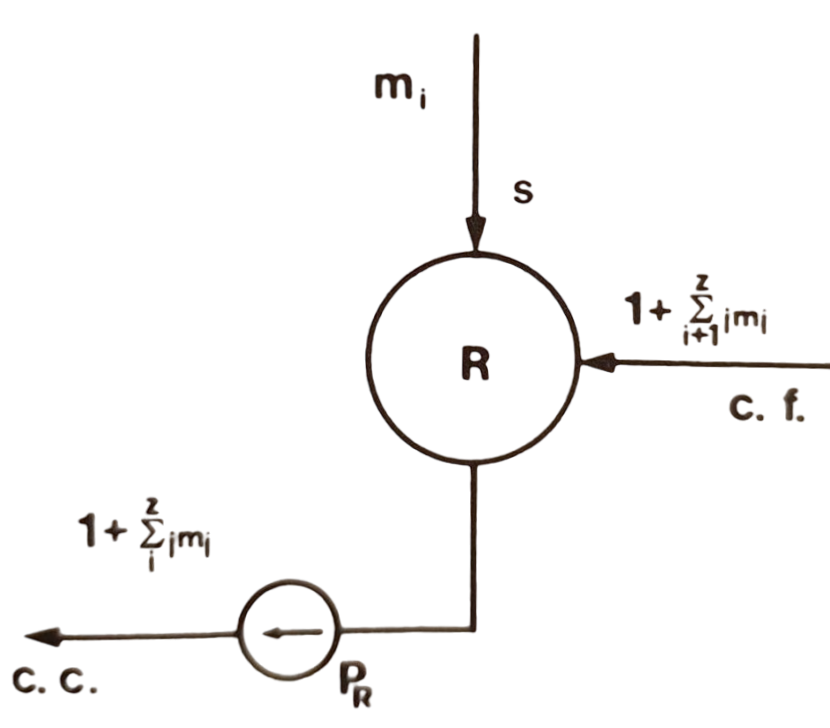
\includegraphics[width=0.3\linewidth]{immagini/miscelatore}
			\label{fig:miscelatore}
		\end{figure}
		
		
		\item \textbf{A superficie}: di tubo in tubo o a fascitubieri.
		
		Non è necessario che i due fluidi si trovino alla stessa pressione.
		
		A valle dello scambiatore è possibile inserire delle valvole di laminazione che permettano di portate il liquido in passaggio di fase alla pressione dello spillamento successivo, oppure si possono usare pompe che elaborino soltanto la portata dello spillamento: entrambe queste alternative sono economicamente abbordabili.
		
		\begin{figure}[H]
			\centering
			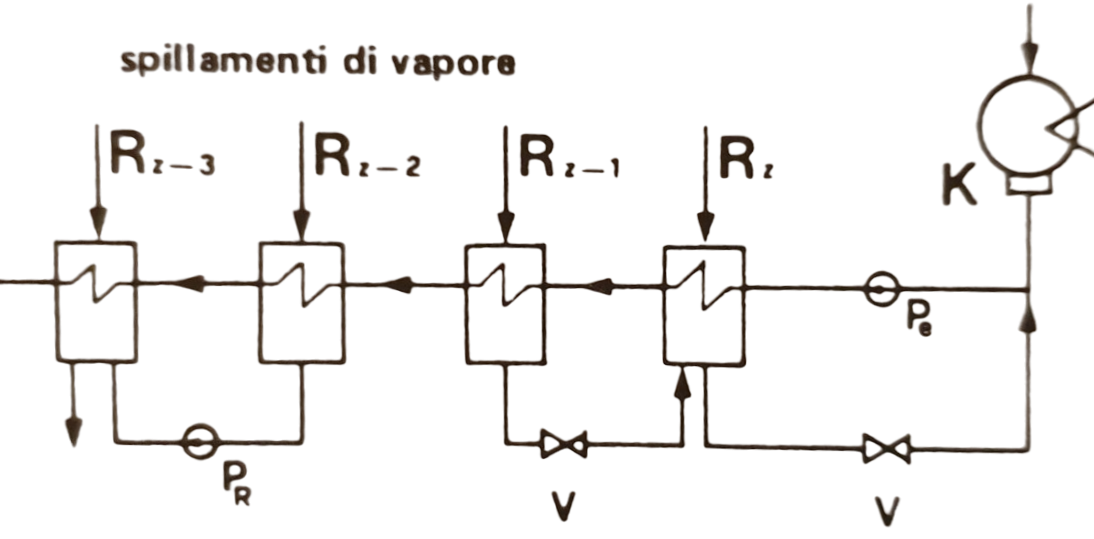
\includegraphics[width=0.5\linewidth]{immagini/rigeneratore}
			\label{fig:rigeneratore}
		\end{figure} 		
	\end{itemize}
	
	Generalmente si adopera un rigeneratore a miscela mentre gli altri rimangono a superficie. 
	
	Il rigeneratore a miscela è sempre presente perché all'interno dell'impianto si raggiungono pressioni sub atmosferiche, ciò significa che potrà entrare dell'aria all'interno delle condotte che andrà in soluzione con l'acqua circolante: i gas disciolti all'interno di un impianto a vapore sono un problema (soprattutto in espansione) perché hanno un comportamento diverso rispetto al vapore; attraverso il degasatore si riesce ad estrarre questi gas dal liquido di lavoro.
	
	Portando l'acqua in condizioni di liquido saturo infatti la solubilità dei gas dispersi nel liquido si annulla ed escono dalla soluzione.
	\begin{figure}[H]
		\centering
		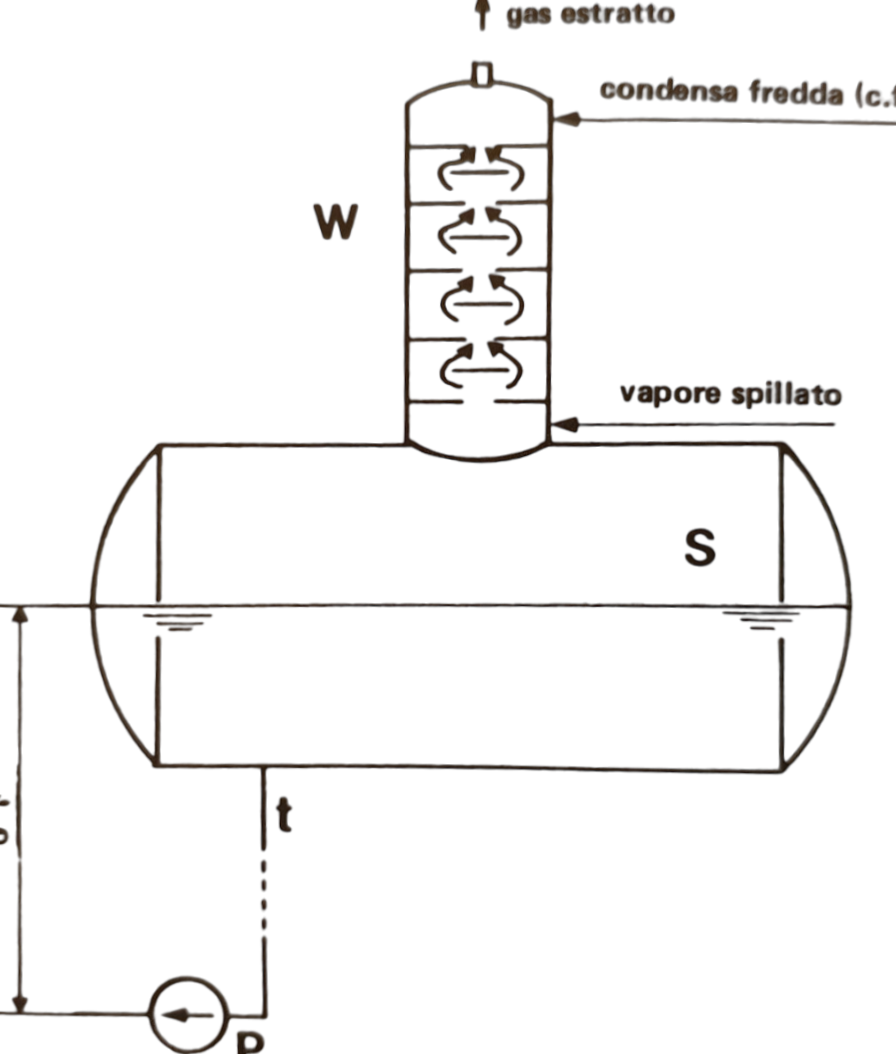
\includegraphics[width=0.4\linewidth]{immagini/degasatore}
		\label{fig:degasatore}
	\end{figure}
	Anche nel condensatore si raggiunge lo stato di liquido saturo, il che potrebbe far pensare di usarlo come degasatore, tuttavia si raggiungono pressioni talmente basse che si dovrebbero usare pompe da vuoto per permettere la separazione dei gas, all'interno del degasatore questo è tranquillamente garantito dalla sovrapressione. \newline 
	
	In ultima analisi, la pompa che estrae il liquido saturo dal degasatore dev'essere posta sottobattente, perché questo è l'unico modo per evitare la cavitazione, infatti dalla classica formula 
	\[NPSH = (P-P_v)-y\]
	La quantità $P-P_v=0$. 	
\end{adjustwidth}


\newpage


\section{Schema impiantistico completo}
	\begin{figure}[H]
		\centering
		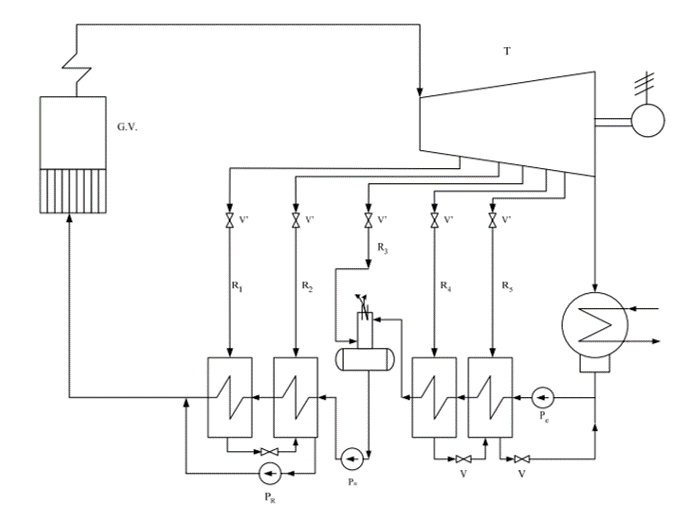
\includegraphics[width=1\linewidth]{immagini/impiantovapore}
		\label{fig:impiantovapore}
	\end{figure}	
\begin{adjustwidth}{2in}{}
	\[R^\text{ott} = {5\over6}\Rightarrow\Delta R^\text{ott} = {1\over6}\]
	La condensa di $R_4,R_5$ viene pompata dalla pompa di estrazione del condensato mentre quella di $R_1, R_2$ dalla pompa $P_R$ e quella di $R_3$ dalla pompa di alimento. 
	
	La  pompa  di  alimento  può essere  azionata,  negli  impianti  più grandi,  mediante uno spillamento di vapore che alimenta una turbopompa di alimento.	
\end{adjustwidth}

\newpage

\section{Elementi di un impianto a vapore}
\begin{figure}[H]
	\centering
	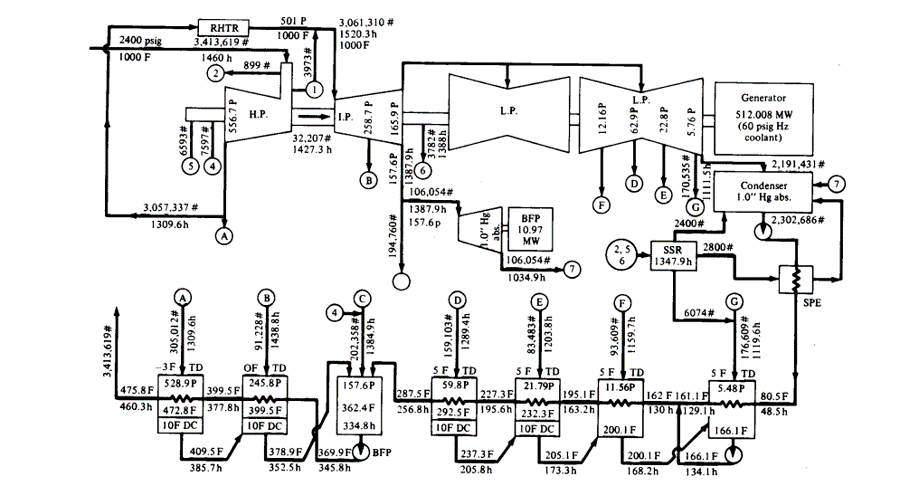
\includegraphics[width=1\linewidth]{immagini/impiantovapore1}
	\label{fig:impiantovapore1}
\end{figure}
\begin{adjustwidth}{2in}{}
	Un impianto reale turbina a vapore presenta una linea di espansione suddivisa in 4 corpi turbina, uno di alta pressione, uno di media pressione e due du bassa pressione a svoluppo speculare, dopodichè è presente una turbina che alimenta tutti gli impianti ausiliari del sistema: tutte le pompe che possono esserci, piuttosto che azionarle con energia elettriva e quindi vincolarle alla frequenza di rete, possono essere alimentate tramite uno spillamento di vapore e quindi avere la libertà di poter variare il numero di giri, e quindi varia la portata elaborata dalle pompe. 
	
	Per quanto riguarda la linea di rigenerazione, qua ci sono  7 rigeneratori di cui uno a miscela ed il rientro delle  condense è semre fatto a pressione più bassa, la condensa viene sempre rimandata al rigeneratore a superficie a pressione più bassa. 
	
	I componenti principali di un impianto a vapore sono

\subsection{Linea di espansione} 
		\begin{figure}[H]
			\centering
			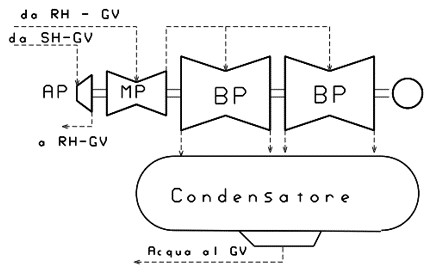
\includegraphics[width=0.3\linewidth]{immagini/impiantovapore2}
			\label{fig:impiantovapore2}
		\end{figure}
		I grandi impianti a vapore, a causa del forte incremento del volume specifico a seguito dell'espansione, presentano più corpi turbina dalle dimensioni via via crescenti. 
\subsection{Turbopompa} che alimenta i sistemi ausiliari
\newpage
\subsection{Scambiatori di calore}
		\begin{itemize}
			\item \textbf{Degasatore}
			\item \textbf{Rigeneratore a superficie} 
			\begin{figure}[H]
				\centering
				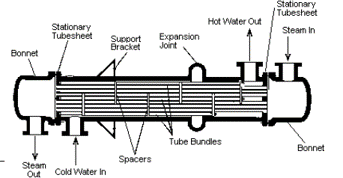
\includegraphics[width=0.5\linewidth]{immagini/rigeneratore1.png}
				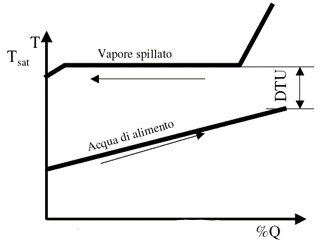
\includegraphics[width=0.3\linewidth]{immagini/rigeneratore2}
				\label{fig:rigeneratore1}
			\end{figure}
			I parametri fondamentali che caratterizzano  la grandezza dello scambiatore per una determinata potenza termica da smaltire sono le differenze di  temperature, prima fra tutte è quella di Pinch Point $\Delta T_{PP}$ che è la minima realizzabile, per cui a pare potenza, ridurre la temperatura di PP consente di aumentare la quantità di calore che viene recuperata ma al tempo stesso comporta un  costo aggiuntivo dovuto all'incremento di superficie dello scambiatore stesso. 
			
			Il vapore spillato si ritrova alla fine dello scambiatore sempre come condensa, per il  repupero di questa condensa si possono percorrere due alternative, o laminare e mandare a pressione inferiore, oppure pompare fino alla pressione superiore. 			
		\end{itemize}
\subsection{Generatore di vapore}
		Il generatore di vapore viene utilizzato per un ampia vastità di impieghi, dalle centrali termoelettriche alla propulsione navale fino alla trazione ferroviaria passando per applicazioni industriali. 
		\begin{figure}[H]
			\centering
			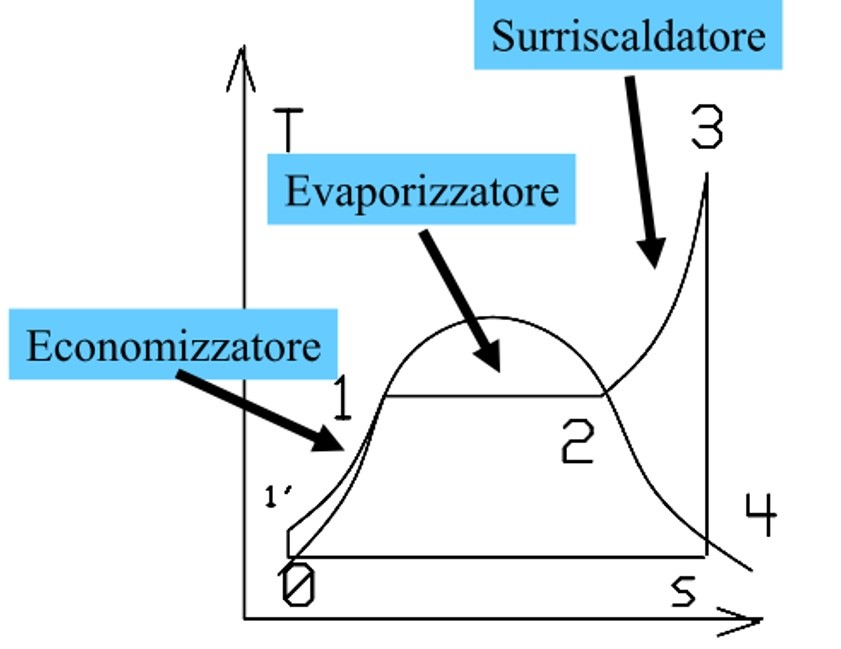
\includegraphics[width=0.3\linewidth]{immagini/impiantovapore3.2}
			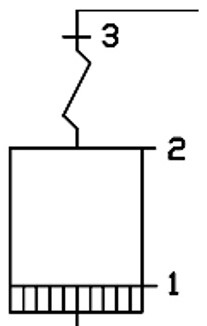
\includegraphics[width=0.1\linewidth]{immagini/impiantovapore3}
			\label{fig:impiantovapore3}
		\end{figure}		
		Le zone della caldaia sono suddivise in base allo stato fisico del fluido:
		\begin{enumerate}
			\item Economizzatore (ECO): stato liquido
			\item Evaporizzatore (EV): Passaggio di fase
			\item Surriscaldatore (SH): stato vapore surriscaldato
			\item Risurriscaldatore (RH): stato vapore surriscaldato
		\end{enumerate}  
\newpage
		si sono 3 principali tipi di generatori di vapore

\subsubsection{Caldaie a grande corpo} 
\subsubsection{Caldaie a tubi di fumo}
			\begin{figure}[H]
				\centering
				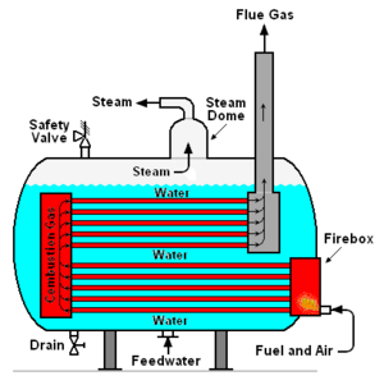
\includegraphics[width=0.3\linewidth]{immagini/GeneratoreVapore}
				\label{fig:generatorevapore}
			\end{figure}
			
			Un involucro contiene l'acqua scaldata da tubi al cui interno passano i prodotti della combustione
\subsubsection{Caldaie a tubi d'acqua}
			\begin{figure}[H]
				\centering
				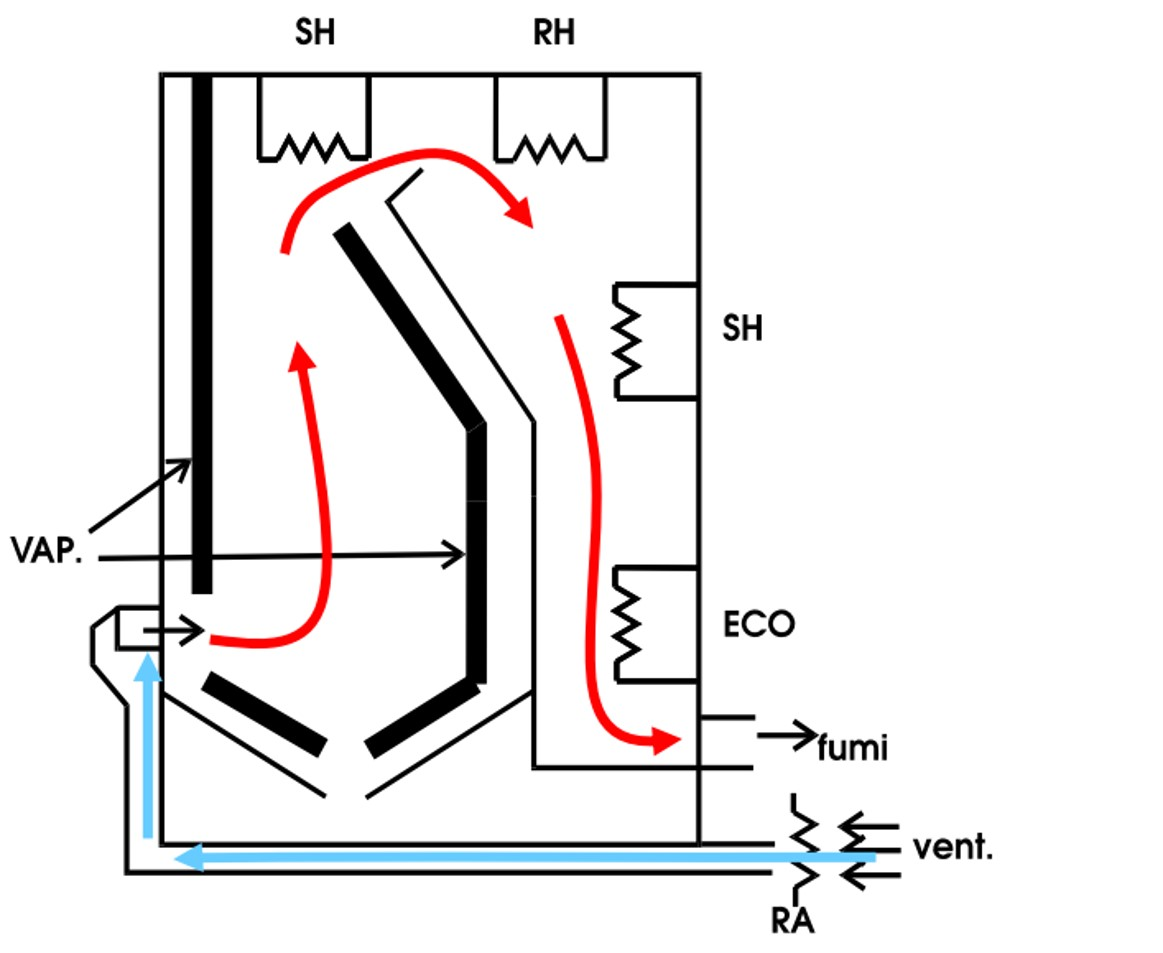
\includegraphics[width=0.5\linewidth]{immagini/Immagine12}
				\label{fig:immagine12}
			\end{figure}			
			Nell'ambiente principale si sviluppa il circuito aria-fumi mentre l'acqua 
			
			Qual è il senso della disposizione degli elementi della caldaia? 
		
			Cosa incontrano i fumi? 
			\begin{figure}[H]
				\centering
				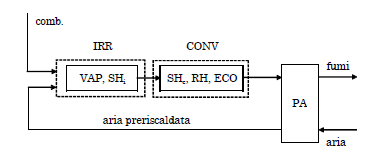
\includegraphics[width=0.5\linewidth]{immagini/GeneratoreVapore1}
				\label{fig:generatorevapore1}
			\end{figure}
			Questi dapprima incontrano la zona irraggiata composta dal vaporizzatore e da un primo surriscaldatore irraggiato e poi incontrano la zona convettiva, composta dal surriscaldatore convettivo, l'eventuale risurriscaldatore e poi l'economizzatore. \newline 
			
			L'acqua, se dovesse seguire il percorso dei fumi, presenterebbe un andamento simile 
			
			DISEGNO DIAGRAMMA TQ "sbagliato"
			
			E non è affatto la situazione ottimale perché se l'obiettivo è quello di minimizzare la differenza di temperatura media, si cerca un andamento del genere
			
			DISEGNO DIAGRAMMA TQ "giusto"
			
			L'acqua allora segue un percorso diverso.
			\begin{figure}[H]
				\centering
				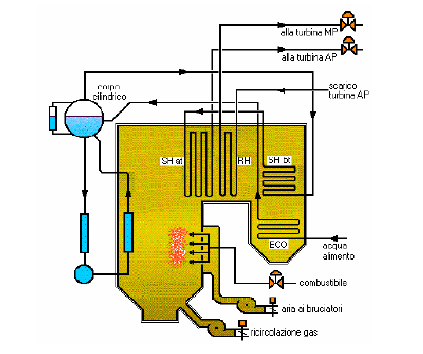
\includegraphics[width=0.6\linewidth]{immagini/GeneratoreVapore2}
				\label{fig:generatorevapore2}
			\end{figure}
			All'interno dei tubi è convogliata all'economizzatore, poi verso il corpo cilindrico all'interno del vaporizzatore, e poi ai relativi surriscaldatori. \newline 
			
			Il motivo di questa disposizione dei circuiti di aria e dei fumi ha una motivazione tecnologica, di resistenza dei materiali
			\begin{figure}[H]
				\centering
				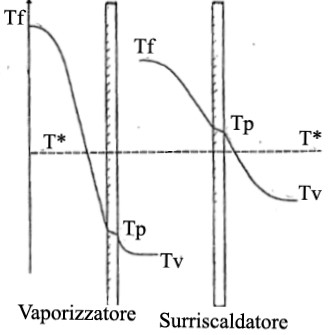
\includegraphics[width=0.3\linewidth]{immagini/GeneratoreVapore3}
				\label{fig:generatorevapore3}
			\end{figure}
			Siano $T_f, T_v, T_P$ le temperature rispettivamente dei fumi, del vapore e della parete, e $T^*$ la temperatura di resistenza del materiale del tubo. 
			
			Si pone il vaporizzatore nella zona più a temperatura più alta perché il coefficiente di scambio termico del vapore in passaggio di fase è 1o volte maggiore del coefficiente di scambio termico del vapore surriscaldato;
			e ciò consente di avere sulla parete una temperatura inferiore a quella di resistenza del materiale. 
			
			Infatti dal fatto che il calore che fluisce dev'essere costante
			\[Q = hS\Delta T\]
			Allora $h\gg\Rightarrow\Delta T\ll$ e la maggior parte del salto di temperatura viene eseguito lato fumi. 
			
			Se questa disposizione non fosse rispettata, si avrebbero da una parte sempre i fumi mentre dall'altra vapore surriscaldato e i due coefficienti di scambio termico si equivarrebbero e questo comporterebbe una temperatura all'interfaccia maggiore di quella di resistenza del materiale. 			
			
			Si pone il vaporizzatore nella parte a temperatura più alta, dove c'è sia irraggiamento che convezione; il profilo di temperatura si disegna partendo da una temperatura dei fumi molto maggiore di quella di resistenza del materiale. 
			
			Quindi per mettere il surriscaldatore è necessario aspettare che la temperatura dei fumi si sia abbassata e si sarà certi che la temperatura di parete sarà al di sotto di quella di resistenza del materiale. 
			 						
			\subsubsection{Circuito Aria-Fumi}
			Sono possibili due soluzioni differenti:
			\begin{itemize}
				\item A caldaia pressurizzata se un solo ventilatore è posto all'ingresso del circuito.
				\item A tiraggio bilanciato se vi sono due ventilatori, uno all'ingresso e uno in uscita. \\
				Questa soluzione consente una movimentazione dell'aria  e dei fumi più efficace ma anche un onere aggiuntivo dovuto alla compressione dei fumi caldi in uscita che richiederanno un lavoro specifico maggiore dell'aria fredda che può essere spinta in ingresso. 
				\item Il preriscaldatore di tipo \textit{Ljungström} è importante perchè consente di aumentare  l'eficienza del generatore di vapore in quanto consente di preriscaldare  l'aria in ingresso a discapito dei fumi in uscita. 
				
				La presenza di questo preriscaldatore è tanto più importate quanto più è alto i grado dirigenerazione, perchè  ad un grado di rigenerazione più alto corrisponde un'ingresso dell'acqua all'economizzatore a temepratura più elevata e quindi presumibilimente  dall'altro lato usciranno dei fumi a temepratura più elevata, quindi per abbassare  la temperatura dei fumi e quindi aumentare l'efficienza del generatore di vapore si usa questo preriscaldatore. 
				
				Dato che i due flussi non possono essere miscelati e il coefficiente convettivo degli stessi risulta modesto (si parla senza perdite di generalità di uno scambio termico aria-aria) questo sistema sfrutta l'elevata capacità termica del materiale col quale è costituito (solitamente materiali ceramici), questo recuperatore è formato da un cilindro di grandi dimensioni rotante attorno al proprio asse. Esso contiene pacchi di lamierini che, per effetto della rotazione del mantello cilindrico, vengono investiti dai fumi caldi e successivamente dall'aria fredda alla quale cedono il calore che hanno immagazzinato dai fumi. 
				\begin{figure}[H]
					\centering
					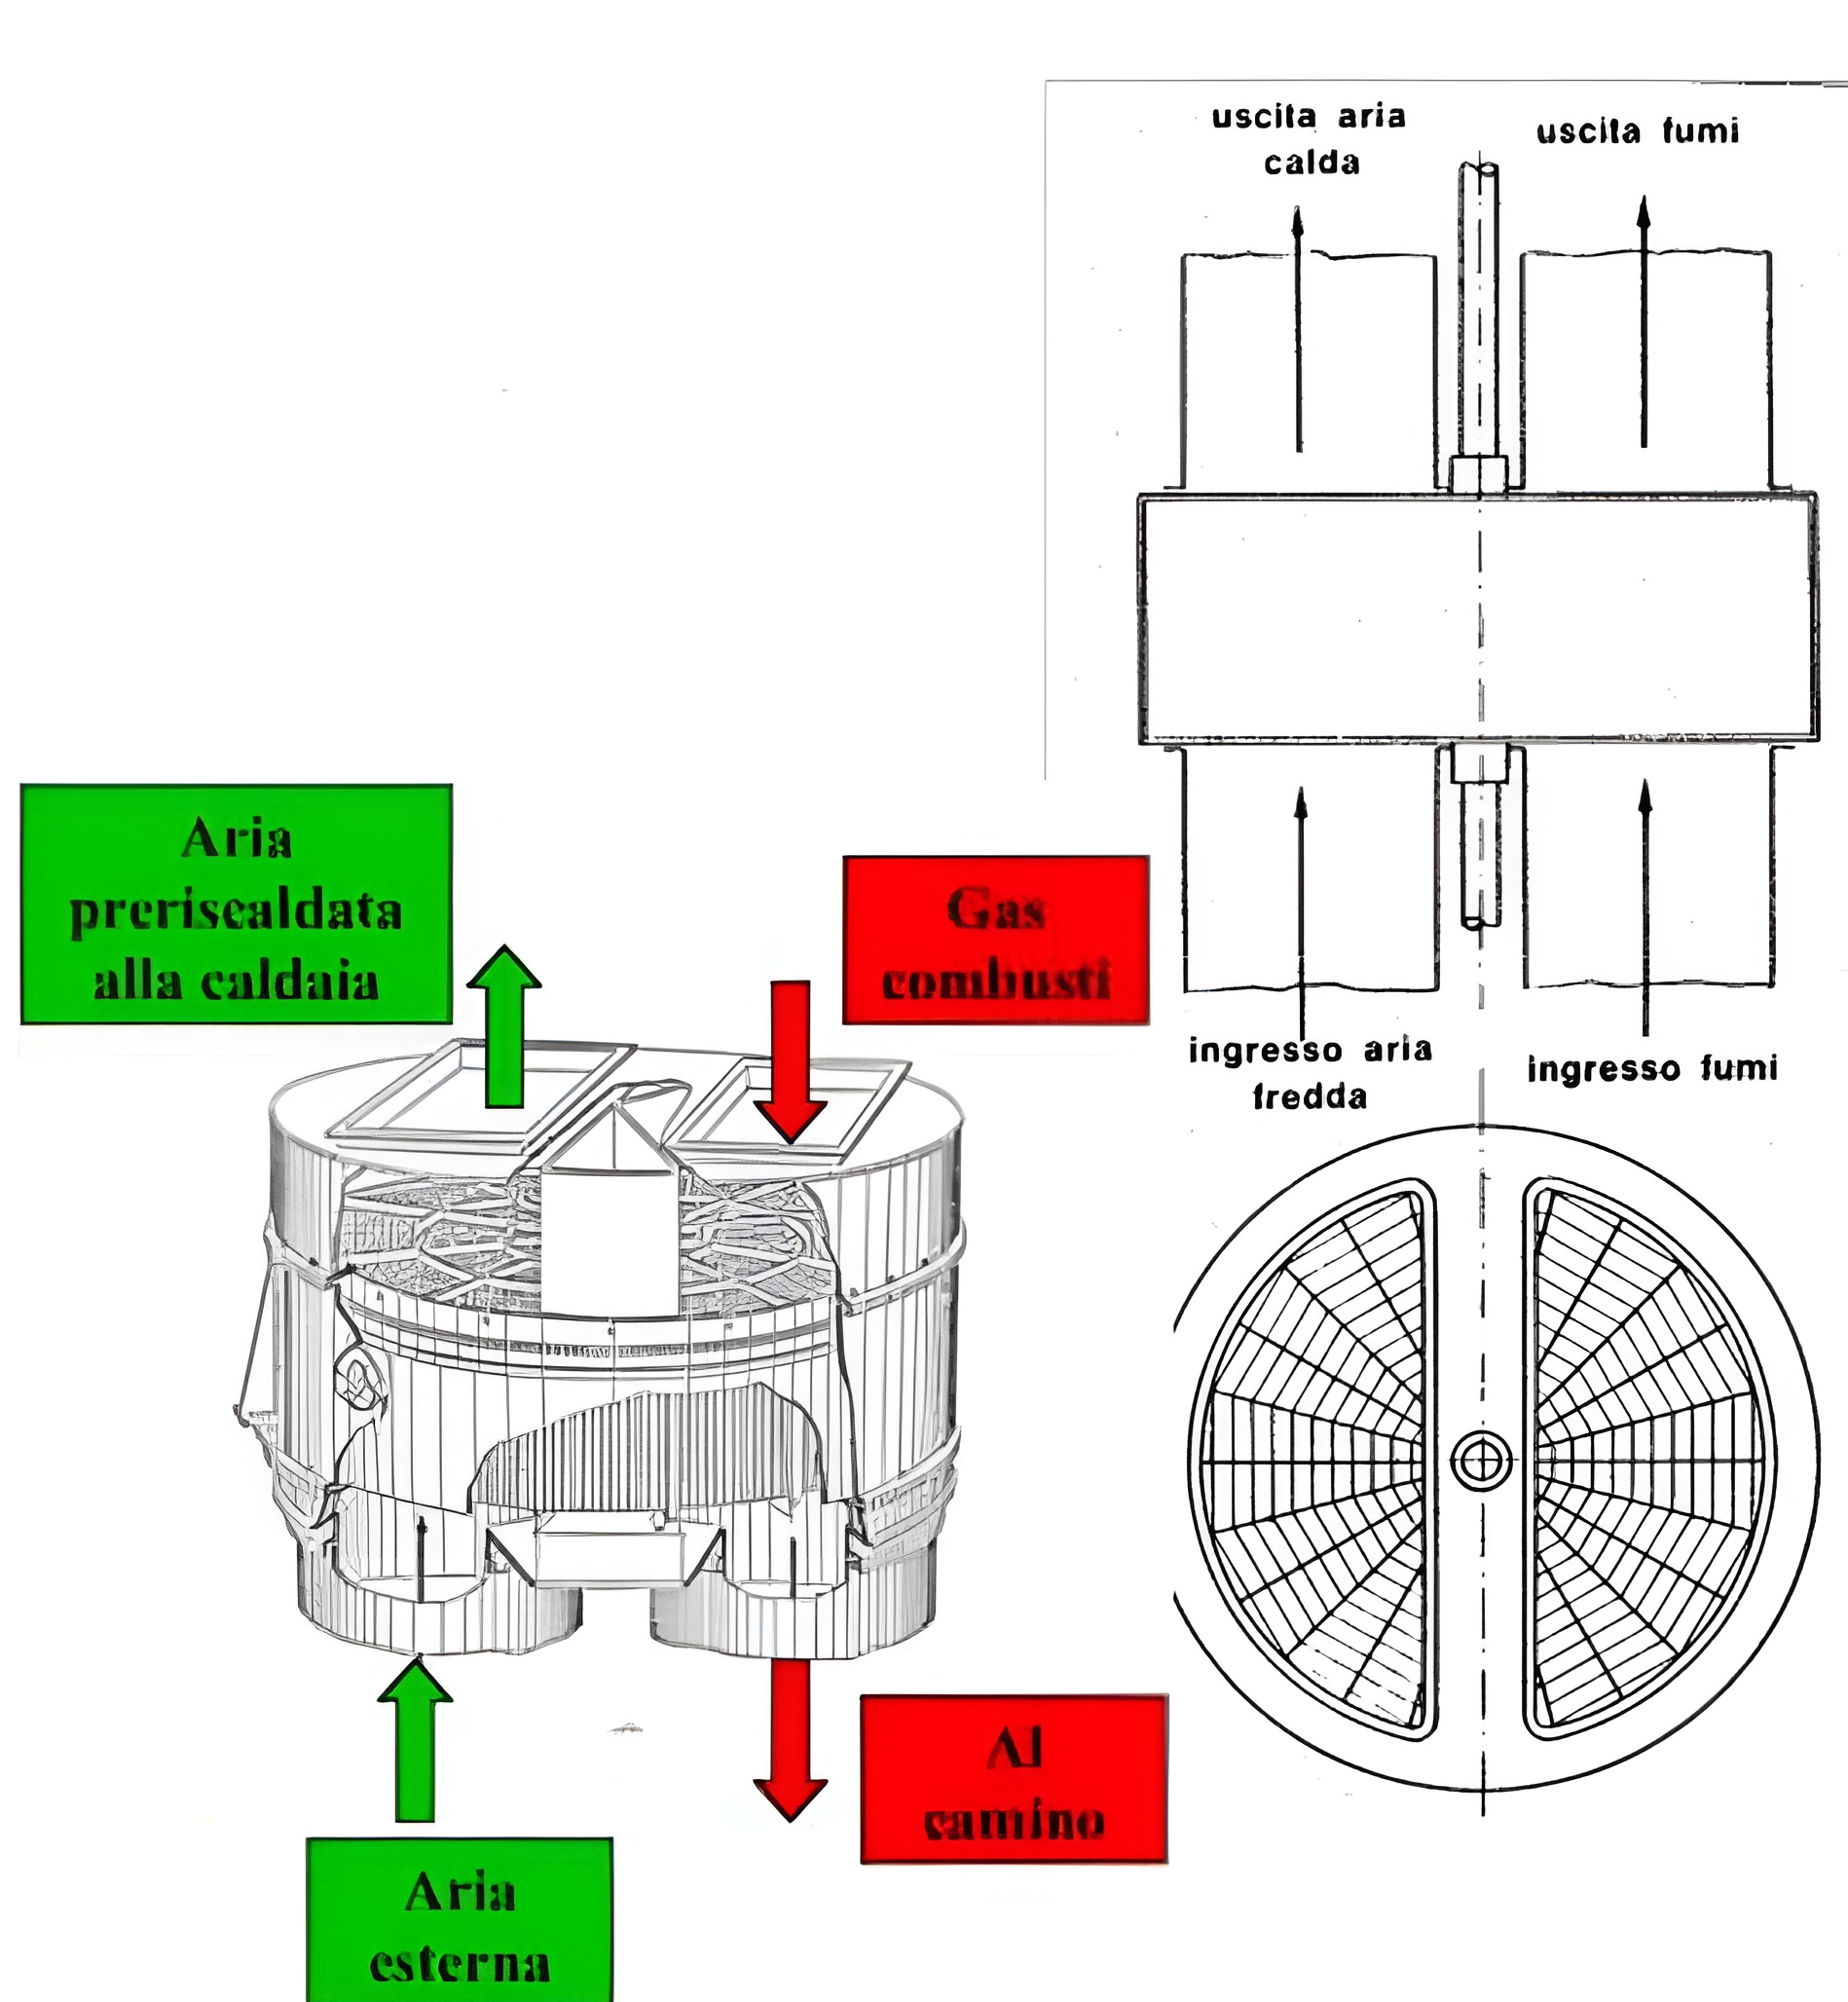
\includegraphics[width=0.3\linewidth]{immagini/Immagine14}
					\label{fig:immagine14}
				\end{figure}
								
				\item Il recuperatore a superficie, a piastre è un'altra soluzione percorribile in alternativa al \textit{Ljungström}, si utilizzano per impianti più piccoli perché per impianti di notevoli dimensioni richiederebbero un ingombro troppo elevato.
			\end{itemize}
			
			\subsubsection{Circuito Acqua-Vapore}
			Ormai è più che noto che il circuito acqua-vapore si suddivida in diversi elementi come economizzatore (costituito da fasci tubieri alettati), evaporatore, surriscaldatore e risurriscaldatore, questi - come visto - suddivisi tra loro perché le caratteristiche fisiche del fluido  all'interno di ogni singolo elemento sono diverse. 
			
			Si è già visto che l'evaporatore, avendo un coefficiente di scambio termico molto maggiore rispetto al surriscaldatore, viene messo a contatto  coi fumi nella parte più calda del generatore di vapore.\newline
			
			Fin'ora però dalla trattazione ci si è dimenticati di menzionare un componente di vitale importanza per il generatore di vapore: il \textbf{Corpo Cilindrico}. 
			
			Questo è un contenitore che riceve in input la miscela acqua-vapore in uscita dall'evaporatore e il liquido saturo in uscita dall'economizzatore e per gravità separa la fase liquida dalla fase vapore, a questo punto pescando da basso si ritrova liquido da mandare all'evaporatore e pescando dall'alto si prende il vapore da mandare al surriscaldatore.
			
			Inoltre il corpo cilindrico assolve anche un'importante funzione "polmone", ovvero di regolazione di portata di vapore in caso ce ne fossero fluttuazioni. \newline
			
			Importante specificare che il corpo cilindrico ha senso d'esistere solamente per pressioni subcritiche, per pressioni supercritiche infatti, non essendoci differenza di densità tra fase liquida e fase vapore, il corpo cilindrico viene sostituito da un altro fascio tubiero, questo tuttavia  comporta la necessità di inserimento di una pompa che faccia circolare il fluido all'interno dell'evaporatore. 
			
			\subsubsection{Tipi di circolazione}
			\begin{itemize}
				\item \textbf{Circolazione naturale}\\
				In una configurazione subcritica, quindi con corpo cilindrico, è possibile sfruttare il cosiddetto "effetto termosifone": la  forza  fluidomotrice è assicurata  dalla  differenza  di pressione  idrostatica,  legata  alla spinta di galleggiamento. 
				
				Man mano che l'acqua riceve calore, avrà una percentuale di vapore sempre maggiore, e quindi questo diminuirà  la densità media e si produrrà la spinta che  fa salire l'acqua che si scalda e mantiene in movimento il circuito dell'evaporatore. 
				
				\item \textbf{Circolazione assistita}\\
				La differenza di densità tra vapore e liquido saturo si riduce mano a mano che ci si avvicina (per poi annullarsi) alle condizioni critiche, ciò comporta che anche i dei generatori di vapore subcritici, nonostante la circolazione sia garantita dall'effetto "termosifone", è necessario installare una pompa che aiuti il fluido in questo attraversamento. 
				
				I tubi dei vari componenti del generatore di vapore sono posti verticalmente.  
				
				\item \textbf{Circolazione forzata}\\
				Una volta arrivati alla pressione critica non esiste più differenza di densità tra vapore e liquidi e quindi si passa ad una configurazione di circolazione forzata: sparisce il corpo cilindrico ed il sistema è tutto alimentato tramite una pompa.
				
				Il generatore di vapore avrà caratteristiche totalmente differenti da quanto visto fin'ora che decretano costi di vapore più elevati. 
			\end{itemize}			
\end{adjustwidth}